\documentclass[12pt]{memoir}

\usepackage[brazil]{babel}
\usepackage[T1]{fontenc}
\usepackage[utf8]{inputenc}
\usepackage{amsfonts, enumitem, tikz, pdfpages, parskip}

\newcommand{\hh}{$\mathcal{H}$}
\newcommand{\pk}{$\mathcal{P}_k$}
\newcommand{\sk}{$\mathcal{S}_k$}
\newcommand{\hash}[2][]{\mathcal{H}^{#1}(#2)}
\newcommand{\concat}{\, \vert \vert \,}
\newcommand{\binwds}[1]{\{0, 1\}^{#1}}
\newcommand{\length}[1]{\vert #1 \vert}

\DeclareMathAlphabet{\mathcal}{OMS}{cmsy}{m}{n}

\def\precircle{(0.00, 0) circle (1.25cm)}
\def\seccircle{(1.75, 0) circle (1.25cm)}
\def\colcircle{(1.75, 0) circle (0.75cm)}

\colorlet{circle edge}{black!50}
\colorlet{circle area}{black!35}

\tikzset{
  filled/.style={fill=circle area, draw=circle edge, thick},
  outline/.style={draw=circle edge, thick}
}

\begin{document}

\chapter{Introdução}

A aplicação de protocolos criptográficos é essencial no contexto da validação e
proteção de quaisquer comunicações realizadas por um conjunto de entidades,
sejam estas dispositivos eletrônicos ou indivíduos, em virtude da possível
criticalidade e sensibilidade atribuídas aos dados transmitidos. Esquemas de
assinatura digital são comumente utilizados para assegurar este processo de
maneira formal \cite{Goldreich:2004:FCV:975541}, através da autenticidade e
não-repúdio do remetente e certeza da integridade dos dados em, a fim de
traduzir o resguardo provido por uma assinatura de próprio punho no mundo real.

Na prática, a maior parte destes esquemas utilizam como alicerce algorítmico
criptossistemas assimétricos baseados em problemas `'difíceis`' da teoria
dos números, como a fatoração de inteiros ou resolução do logaritmo discreto,
ambos para números grandes. Este fato provê a segurança necessária para os
esquemas em computadores clássicos (eletrônicos), por conta da inexistência de
algoritmos que resolvem estes problemas em tempo polinomial, até o momento.
Entretanto, em computadores quânticos, algoritmos dessa forma já existem - em
especial, o algoritmo de Shor \cite{Shor:1997:PAP:264393.264406} - efetivamente
tornando estes esquemas clássicos inseguros neste novo contexto.

Para combater esta situação, a criptografia pós-quântica encarrega-se de buscar
algoritmos criptográficos cuja segurança é considerada suficiente mesmo
utilizando-se de um computador quântico e ataques especializados, como o
algoritmo de Grover \cite{Grover:1996:FQM:237814.237866}. Esta área conta com
diversas abordagens diferentes: a criptografia baseada em reticulados,
polinômios multivariados sobre um corpo finito, códigos de correção de erros,
morfismos entre curvas elípticas supersingulares e criptossistemas simétricos.
Entretanto, reduções de segurança formais não existem para alguns destes
métodos, e para outros, o tamanho das chaves impossibilita a utilização destes
em aplicações práticas.

Não obstante, uma abordagem distinta de esquema de assinatura digital
resistente a computadores quânticos pode ser obtida apenas com funções de
resumo criptográfico, construídas a partir de funções de mão única
\cite{cryptoeprint:2005:328}. De fato, estas funções, desde que apresentem
requisitos de segurança como resistência à segunda pré-imagem e à colisões, são
necessárias e suficientes para a construção de esquemas bem comportados e
seguros \cite{Rompel:1990:OFN:100216.100269}. Visto que estas funções são
estudadas exaustivamente por conta de sua vasta presença em diversos âmbitos da
segurança da informação, reduções de segurança são mais comuns em relação a
outras abordagens pós-quânticas, e tamanhos de chaves e assinaturas não são
proibitivos.

Esquemas de assinatura digital baseados em funções de resumo criptográfico
consistem da utilização de um esquema de assinatura digital única, onde apenas
uma mensagem pode ser assinada de modo seguro, ou sua combinação com a
estrutura de dados chamada de árvore de Merkle
\cite{Merkle:1989:CDS:118209.118230}, que abriga diversos pares de chave do
esquema supracitado como suas folhas, e reduz a verificação destes para uma
única chave, codificada em sua raiz. Esta árvore é construída com a
concatenação de resumos criptográficos do conteúdo dos nós, habilitando assim a
assinatura de diversas mensagens. Como uma função específica não é necessária,
é possível obter uma grande variedade de esquemas, garantindo a versatilidade
destas abordagens.

Embora os esquemas iniciais tenham sido construídos sem atenção particular à
eficiência de modo geral (e.g. o esquema de assinatura única de Lamport-Diffie
\cite{Lamport1979} assina apenas um \emph{bit} de informação em sua forma mais
simples), muitos resultados práticos demonstram a redução contínua do tempo de
verificação da assinatura, tamanho e tempo para geração do par de chaves e
assinatura, bem como avanços teóricos possibilitam a utilização de funções com
requisitos de segurança mínimos, garantem o conceito de sigilo encaminhado
\cite{Buchmann:2011:XPF:2184003.2184011} (i.e. comprometimento de uma chave não
implica na segurança de mensagens que utilizaram esta chave anteriormente) e da
ausência de estado \cite{Bernstein2015} (i.e. esquema não necessita registrar
quais chaves de assinatura única já foram utilizadas).

Neste trabalho, será estudada bibliografia referente aos temas abordados,
buscando encontrar as vantagens e desvantagens de cada um dos esquemas
de assinatura digital escolhidos, bem como observar seu desempenho e tamanho
de elementos como par de chaves e assinatura, ao utilizar funções de resumo
criptográfico distintas em implementações produzidas ou fornecidas.
Elaborar-se-á uma comparação exaustiva dos esquemas de assinatura única e
baseados em árvores de Merkle a fim de demonstrar a evolução recorrente
destes algoritmos.

\section{Objetivos}

\begin{itemize}

  \item \emph{Objetivo geral.} Apresentar um estudo detalhado sobre esquemas
    de assinatura digital baseados em funções de resumo criptográfico,
    partindo de esquemas de assinatura única \cite{Lamport1979}, observando
    o refinamento destes, até o estado da arte, onde não é necessário saber
    quantas assinaturas foram geradas anteriormente \cite{Bernstein2015}, bem
    como implementações em linguagem de alto nível para a fácil compreensão
    destes esquemas.

  \item \emph{Objetivos específicos.} Descrever os esquemas de assinatura
    digital única Lamport-Diffie e Winternitz, e variantes; descrever os
    esquemas de assinatura digital baseado em árvores de Merkle: \emph{Merkle
    Signature Scheme}, \emph{eXtended Merkle Signature Scheme}, SPHINCS;
    implementar os esquemas supracitados; comparar o desempenho destes,
    utilizando funções de resumo criptográfico e parâmetros internos aos
    algoritmos distintos, onde aplicável.

\end{itemize}

\chapter{Primitivas criptográficas}

Neste capítulo, são mostradas breves explicações sobre os conceitos
necessários a fim de entender inteiramente um esquema de assinatura digital:
a função de resumo criptográfico, utilizada para que o processo de assinatura
seja menos custoso e mais seguro, e um exemplo da construção teórica por trás
deste tipo de função; os conceitos de criptografia simétrica e assimétrica, e
uma simples comparação entre os mesmos, com foco na variante assimétrica,
novamente apresentando um exemplo comum -- mas não resistente a computadores
quânticos -- e, por fim, a definição formal de um esquema de assinatura digital
agregando estas noções.

\section{Funções de resumo criptográfico}

Uma função de resumo \hh{} mapeia valores deterministicamente entre dois
conjuntos. O domínio pode ter tamanho infinito, e neste caso a função pode ser
chamada de função de compressão; a imagem deve ser estritamente menor do que o
domínio e finita, e elementos deste conjunto são chamados de resumos. É
desejável para \hh{} que estes mapeamentos ocorram de tal maneira que não
ocorra uma relação aparente entre entradas e saídas da função. Funções de
resumo adicionadas de propriedades que tornam-as adequadas para utilização no
contexto de segurança da informação são chamadas de funções de resumo
criptográfico, e possibilitam a certeza da integridade de dados, mesmo que
armazenados em um dispositivo inseguro.

Tome $X : \binwds{*}$ e $Y : \binwds{n}$, $n \in \mathbb{N}$. Então,
$\mathcal{H} : X \longrightarrow Y$. De acordo com
\cite{stinson2005cryptography}, para que qualquer \hh{} seja considerada
criptográfica, deve ser difícil resolver os três problemas listados abaixo.
É importante notar que um problema é considerado `'difícil`', ou
computacionalmente impraticável, quando o tempo ou recursos gastos para esta
computação excedem a validade ou utilidade da informação desejada.

\begin{enumerate}[label=\roman*.]

  \item Fornecido um resumo $h \in Y$, achar a mensagem original $m \in X$ que
    gerou $h$ através de $\hash{m} = h$; \hh{} é considerada resistente à
    pré-imagem (\textsc{Pre}) se isto não pode ser resolvido de maneira
    eficiente.

  \item Fornecida uma mensagem $m_0 \in X$, achar uma mensagem $m_1 \in X$ tal
    que $m_0 \neq m_1$ e $\hash{m_0} = \hash{m_1}$. \hh{} é considerada
    resistente à segunda pré-imagem (\textsc{Sec}) se isto não pode ser
    resolvido de maneira eficiente.

  \item Para quaisquer duas mensagens $m_0, \; m_1 \in X$ e $m_0 \neq m_1$,
    $\hash{m_0} = \hash{m_1}$. \hh{} é considerada resistente à colisões
    (\textsc{Col}) se isto não pode ser resolvido de maneira eficiente.

\end{enumerate}

Note que \textsc{Sec} e \textsc{Col}. apresentam uma sutil diferença: no
primeiro, um adversário não pode escolher $m_0$, enquanto no segundo, quaisquer
pares de mensagens podem ser testados. A resistência à colisão, portanto,
implica na resistência à segunda pré-imagem, visto que basta um adversário
fixar $m_0$ para simular o cômputo de $m_1$. Outra característica desejada é o
efeito avalanche, baseado no conceito de difusão
\cite{Stallings:2010:CNS:1824151}: trocar apenas um \emph{bit} da mensagem $m$
deve modificar cerca de metade dos \emph{bits} do resumo, e vice-versa.

\begin{figure}[h]
  \centering
  \begin{tikzpicture}
    \begin{scope}[fill opacity=0.5]
      \clip \precircle;
      \fill[filled] \seccircle;
      \fill[filled] \colcircle;
    \end{scope}
    \draw[outline] \precircle node {\textsc{Pre}};
    \draw[outline] \seccircle node {};
    \draw node[right=1.75cm, above=0.75cm] {\textsc{Sec}};
    \draw[outline] \colcircle node {\textsc{Col}};
  \end{tikzpicture}
  \caption{Diagrama de Venn das resistências de uma função de resumo
    criptográfico.}
  \label{fig:1}
\end{figure}

Na Figura \ref{fig:1}, estão destacados os requisitos comuns para a utilização
de funções de resumo criptográfico no contexto de esquemas de assinatura
digital, em vista da possibilidade de uma entidade maliciosa, geralmente
chamada de adversário, desejar produzir assinaturas forjadas. É possível
constatar que, embora exista uma divisão estrita entre \textsc{Pre} e
\textsc{Sec}, observa-se que na prática, é possível assumir que a segunda
implica a primeira resistência \cite{Menezes:1996:HAC:548089}.

Enumeram-se algumas aplicações comuns para estas funções: a verificação da
integridade de um arquivo, i.e. determinar se mudanças neste foram feitas ao
longo de uma transmissão, ou qualquer outro evento; a fim de evitar o
armazenamento de senhas em texto plano, é possível manter apenas o resumo
criptográfico destas, e no momento da autenticação do usuário perante o
serviço, comparar apenas estes resumos\footnote{É possível armazenar tabelas de
resumos pré-computados a fim de atacar serviços que não empregam uma maneira
mais elaborada de autenticação (por exemplo, um valor aleatório
concatenado ao resumo criptográfico da senha do usuário).}; resumos
criptográficos são comumente empregados como identificadores únicos para um
arquivo (e.g. \emph{commits} em um sistema de controle de versões); entre
outras aplicações, como a geração de números pseudoaleatórios.

\subsection{Construção esponja}

A construção esponja \cite{SpongeReference}, de característica iterativa,
permite a generalização de funções de resumo, naturalmente com saídas de
tamanho fixo, para funções com saídas de tamanho arbitrário, baseadas em uma
função interna, geralmente uma permutação $f$ de tamanho fixo $b$. Este valor,
também chamado de largura, é composto da adição da taxa de \emph{bits} $r$ e da
capacidade $c$. Assim, a construção opera em um estado de $b = r + c$
\emph{bits}.

O estado inicial, análogo a um vetor de inicialização no contexto de algoritmos
criptográficos, não necessita de valores especiais e é inicializado com valores
nulos. A entrada $m$ é preenchida com uma função de preenchimento \texttt{pad}
de tal modo que $r \mid \length{m}$, e dividida em blocos de tamanho $r$. A
fase de absorção de $m$ pela esponja procede da seguinte maneira: a operação de
ou exclusivo ($\oplus$) é calculada entre os blocos e os estados da construção,
intercalados por aplicações de $f$.

% TODO: imagem da construção esponja

Ao término do processamento dos blocos, a fase de compressão é iniciada, onde
$n$ blocos de tamanho $r$ compõem a saída da função, novamente intercalados por
aplicações de $f$, onde $n$ é parametrizável pelo usuário. Os últimos $c$ bits
do estado nunca são diretamente afetados pelos blocos, e também nunca revelados
durante a fase de compressão. Essencialmente, estão correlacionados com o nível
de segurança da construção esponja. Assim, uma função esponja pode ser definida
como $\textsc{Sponge}[f, \texttt{pad}, r]$.

A função esponja \textsc{Keccak} \cite{KeccakReference} é definida a partir
desta construção, e pode agir como uma função de resumo criptográfico. Existem
sete permutações passíveis de utilização nesta função: defina $w = 2^{\ell}, \;
\ell \in \{0, \dots, 6\}$.  Estas são chamadas de $\textsc{Keccak}-f[b]$, onde
$b = 25w$, cujo estado $a$ é descrito como uma estrutura tridimensional com
elementos em $\mathbb{F}_2$, de dimensões $5 \times 5 \times w$. Esta
permutação é iterativa e consiste de um número de rodadas $n_R$. Cada rodada
$R$, por sua vez, consiste da composição de cinco etapas: $R = \iota \circ \chi
\circ \pi \circ \rho \circ \theta$.

\begin{enumerate}

  \item[Etapa $\theta$:] Calcula o ou exclusivo entre um elemento de $a$ e
    todos os elementos das colunas adjacentes a este.

  \item[Etapa $\rho$:] Dispersa os elementos entre cortes transversais
    verticais de $a$.

  \item[Etapa $\pi$:] Rearranja elementos em cortes transversais horizontais de
    $a$.

  \item[Etapa $\chi$:] Modifica uma elemento de uma linha de $a$ de acordo com
    uma função não-linear de dois outros bits adjacentes. Análogo a uma caixa-S.

  \item[Etapa $\iota$:] Calcula o ou exclusivo entre o estado $a$ e uma
    sequência gerada por um \emph{linear-feedback shift register} alimentado
    pelo índice da rodada atual, tornando a rodada assimétrica.

\end{enumerate}

Tome \texttt{pad10*1} como uma função que gera palavras que iniciam e terminam
com $1$, e têm número não-negativo de zeros. Formalmente, para uma mensagem
qualquer $m$ e um tamanho de saída $d \in \mathbb{N}^{*}$, a função esponja é
definida como
\begin{equation}
  \textsc{Keccak}[r, c](m, d)
    = \textsc{Sponge}[\textsc{Keccak}-f[r + c], \texttt{pad10*1}, r]
\end{equation}

onde $r$ tem um valor padrão de $1600 - c$. Assim,
\begin{equation}
  \textsc{Keccak}[c] = \textsc{Keccak}[1600 - c, c].
\end{equation}

Finalmente, as funções padronizadas em \cite{Dworkin2015} como a família SHA-3
são definições de \textsc{Keccak} com parâmetros fixos, e.g.
\begin{equation}
  \text{SHA3-}256(m) = \textsc{Keccak}[512](m \; \vert \vert \; 01, 256).
\end{equation}

\section{Criptografia simétrica}

Algoritmos criptográficos que utilizam a mesma chave para criptografar o
texto plano e descriptografar o texto correspondente cifrado são classificados
como algoritmos de criptografia simétrica. A chave representa um segredo
compartilhado entre entidades em uma comunicação segura. Porém, a necessidade
de um canal seguro para o estabelecimento desta chave apresenta-se como uma
desvantagem deste tipo de criptografia. Geralmente, cifras de bloco (DES, AES)
ou de fluxo (RC4, Salsa20) são a base para estes algoritmos. Utilizando estas
como alicerce, é possível construir funções de resumo criptográfico: por
exemplo, a construção Merkle-Damgård, base para as funções MD5, SHA1 e SHA2,
utiliza uma função de compressão única, obtida a partir de uma cifra de bloco.

\section{Criptografia assimétrica}

Em contrapartida, a criptografia assimétrica, ou criptografia de chaves
públicas, engloba os algoritmos que utilizam um par de chaves: a chave privada
(\sk{}), conhecida apenas pela entidade que a gerou, e a chave pública (\pk{}),
distribuída livremente. Isto possibilita o uso livre de \pk{} para a
comunicação segura com o detentor da chave sem a necessidade de um canal
seguro, em virtude da construção dos algoritmos. A segurança destes depende da
``dificuldade'' computacional de determinar uma chave privada a partir da chave
pública, e também do armazenamento de \sk{} em um lugar seguro. Problemas em
teoria de números e álgebra que atualmente não admitem soluções em tempo
polinomial são comumente utilizados como base para algoritmos assimétricos.
Porém, percebe-se que, com a introdução de um computador quântico, estes
problemas podem ser resolvidos de maneira significativamente mais rápida, como
visto em \cite{Shor:1997:PAP:264393.264406}.

\subsection{O criptossistema RSA}

O algoritmo conhecido como RSA \cite{Rivest:1978:MOD:359340.359342} é uma
implementação de criptografia assimétrica amplamente utilizada. É baseado na
dificuldade de fatorar o produto de dois números primos suficientemente
grandes\footnote{O algoritmo é baseado no problema RSA, definido como realizar
uma operação de chave privada no algoritmo RSA utilizando apenas \pk{}.
Acredita-se que este problema seja equivalente à fatoração de inteiros
\cite[3.30]{Menezes:1996:HAC:548089}.}. Em virtude de seu baixo desempenho
computacional, geralmente apenas um resumo criptográfico da mensagem desejada é
codificado por este algoritmo. Abaixo, uma descrição do funcionamento do
algoritmo. Tome $\phi(x)$ como a função totiente de Euler, que representa a
quantidade de números relativamente primos a $x$.

\begin{enumerate}

  \item[] \emph{Geração de chaves.} Gere dois números primos $p, q$
    aleatoriamente, suficientemente grandes e de tamanhos similares. Compute
    $n = p q$ e $\phi(n) = (p - 1) (q - 1)$. Selecione um número aleatório $e$
    relativamente primo a $\phi(n)$. Então, use o algoritmo de Euclides
    estendido para computar $d$ tal que $ed \equiv 1 \pmod{\phi(n)}$), i.e.
    a inversa multiplicativa modular de $e$. Finalmente, $\mathcal{S}_k = d$ e
    $\mathcal{P}_k = (n, e)$.

  \item[] \emph{Codificação.} Obtém-se \pk{} da entidade para qual
    deseja-se criptografar uma mensagem. Transforma-se uma mensagem $m$ em um
    inteiro no intervalo $[0, n - 1]$ através de uma função de preenchimento.
    O texto cifrado $c = m^e \pmod{n}$ é calculado através de um algoritmo
    como a exponenciação quadrática e enviado para a entidade desejada.

  \item[] \emph{Decodificação.} O receptor da mensagem calcula $m = c^d
    \pmod{n}$.

  \item[] \emph{Demonstração}. Para demonstrar $m^{ed} \equiv m \pmod{n}$, é
    suficiente mostrar $m^{ed} \equiv m \pmod{p}$ e $m^{ed} \equiv m \pmod{q}$,
    pelo Teorema Chinês do Resto. Se $m \equiv 0 \pmod{p}$, então
    $gcd(m, p) = p$ e certamente $m^{ed} \equiv 0 \equiv m \pmod{n}$.
    Se $m \not\equiv 0 \pmod{p}$, então $mdc(m, p) = 1$ e pelo Pequeno Teorema
    de Fermat, $m^{p - 1} \equiv 1 \pmod{p}$. Reescrevendo o produto $ed$ como
    $ed = 1 + y\phi(n) = 1 + y(p - 1)(q - 1), \; y \in \mathbb{N}$, então
    \begin{equation}
      m^{ed} \equiv m^{1 + y(p-1)(q-1)} \equiv (m^{p-1})^{y(q-1)}m
        \equiv 1^{y(q-1)}m \equiv m \pmod{p}.
    \end{equation}
    Analogamente, substituindo $p$ por $q$ no argumento acima, tem-se a prova
    que $\forall m \in \mathbb{N}, \; m^{ed} \equiv m \pmod{n}$.

\end{enumerate}

\section{Esquemas de assinatura digital}

Um esquema de assinatura digital é uma construção matemática que habilita a
demonstração de certas propriedades sobre mensagens assinadas: nomeadamente,
a autenticação do remetente, onde esta entidade pode ser facilmente
identificada como a emissora da assinatura digital; a integridade da mensagem,
i.e. a certeza de que esta não foi modificada ao ser transmitida por um canal
possivelmente inseguro; e o não-repúdio do remetente, onde não é possível negar
que uma mensagem foi assinada e enviada, após este fato.

\begin{figure}[h]
  \centering
  \begin{tikzpicture}
    \node (hm) at (-1.25, 0) {$m$};
    \node (in) at (0, -2) {$1^n$};
    \node (sk) at (0, -1) {\sk{}};
    \node (pk) at (4, -1) {\pk{}};
    \node (ds) at (2, 0)
      {\scriptsize{$m \concat \textsc{Sig}(\mathcal{S}_k, \hash{m})$}};
    \node (res) at (5.5, 0) {\scriptsize\{0, 1\}};
    \node[draw] (sig) at (0, 0) {\textsc{Sig}};
    \node[draw] (gen) at (2, -2) {\textsc{Gen}};
    \node[draw] (ver) at (4, 0) {\textsc{Ver}};
    \draw[-latex] (gen) to (1.25, -1) to (sk);
    \draw[-latex] (gen) to (2.75, -1) to (pk);
    \draw[-latex] (sk) -- (sig);
    \draw[-latex] (hm) -- (sig);
    \draw[-latex] (sig) -- (ds);
    \draw[-latex] (ds) -- (ver);
    \draw[-latex] (pk) -- (ver);
    \draw[-latex] (ver) -- (res);
    \draw[-latex] (in) -- (gen);
  \end{tikzpicture}
  \caption{Funcionamento típico de um esquema de assinatura digital.}
  \label{fig:2}
\end{figure}

Esquemas de assinatura digital são fortemente baseados em criptografia de
chaves públicas, e consistem de três algoritmos: a geração de chaves
$\textsc{Gen}(1^n)$, que gera um par de chaves aleatório $(\mathcal{P}_k,
\mathcal{S}_k)$ com parâmetro de segurança $n$; o algoritmo de assinatura
$\textsc{Sig}(\mathcal{S}_k, m)$, que produz uma assinatura $\sigma$ para uma
mensagem $m$; e o algoritmo de verificação $\textsc{Ver}(\mathcal{P}_k, m,
\sigma)$, que retorna o estado de validade da assinatura como um valor verdade
binário. De acordo com \cite{Goldreich2004}, todas as assinaturas geradas por
\textsc{Sig} devem ser verificáveis por \textsc{Ver} utilizando todas as chaves
geradas por \textsc{Gen}. Formalmente, $\forall (p, s) \in
\textsc{Gen}^{\rightarrow}(1^n)$ e $\forall w \in \{0, 1\}^{*}$,
\begin{equation}
    \text{Pr}[\textsc{Ver}(p, w, \textsc{Sig}(s, w)) = 1] = 1.
\end{equation}

Na Figura \ref{fig:2}, é possível visualizar um diagrama do comportamento de
um esquema de assinatura digital genérico. Note que $\sigma$ geralmente é
composto da concatenação da mensagem original com a assinatura do resumo
criptográfico desta, embora a saída do algoritmo \textsc{Sig} consista apenas
da aplicação de uma função interna a este ao resumo.

\anexo
\chapter{Artigo submetido para PQCrypto 2018}
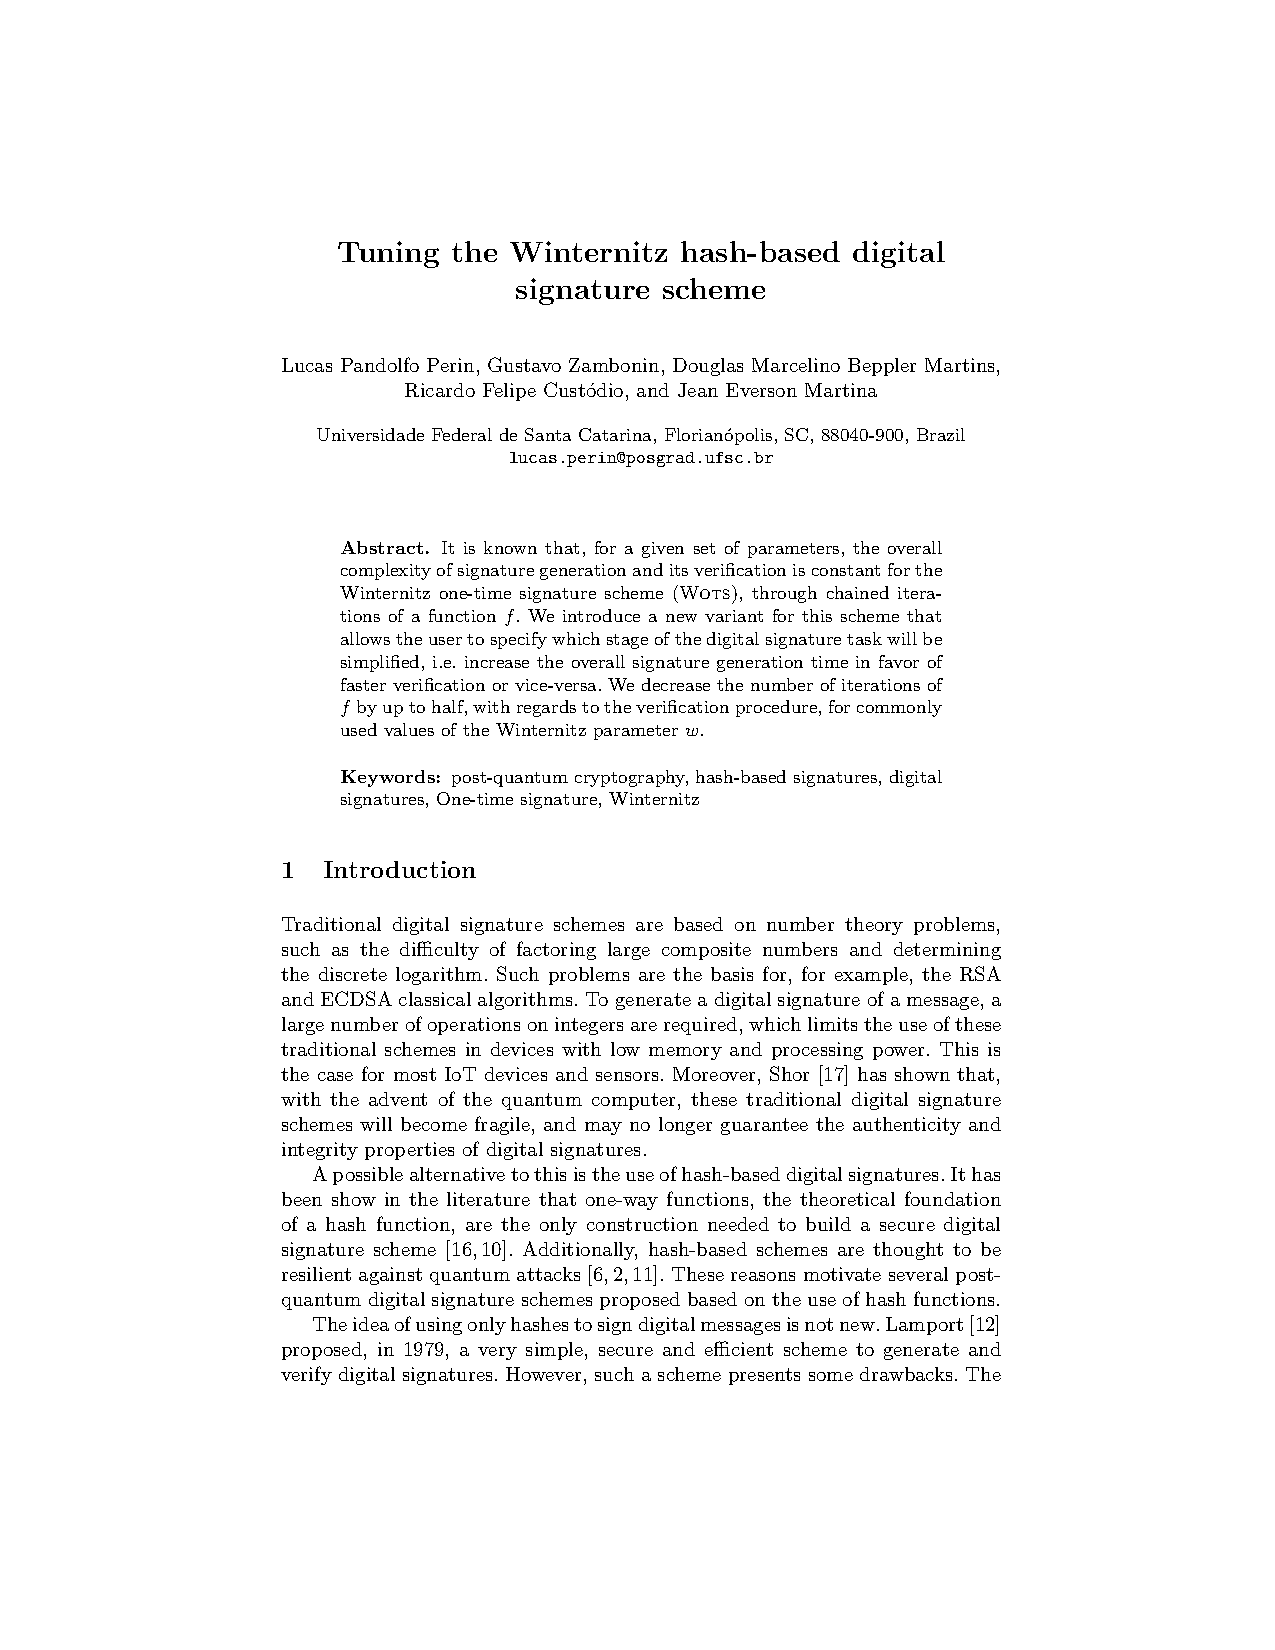
\includepdf[pages=-]{tuning-winternitz}

\bibliographystyle{alpha}
\bibliography{ref}

\end{document}
